%%% Kapitola 1: Analýza existujících řešení

\chapter{Analýza existujících řešení}
\label{chap:related}

Tato kapitola pokrývá teoretické základy Bitcoinu potřebné pro pochopení
zbytku práce, přehled existujících peněženkových aplikací a~analýzu
technických přístupů k~realizaci klíčových funkcí -- zejména komunikace
s~hardwarovou peněženkou, správy multisig peněženek a~koordinace
podepisování. Zaměřujeme se na podporu multisig transakcí, coin control
a~integraci hardwarových peněženek na mobilních platformách.


%%% -----------------------------------------------------------------
\section{Protokol Bitcoin}
\label{sec:bitcoin-basics}

Bitcoin~\citep{Nakamoto08} je decentralizovaný platební systém, který
funguje bez důvěryhodné třetí strany. Podrobný výklad technologie Bitcoinu
by vydal na celou knihu (viz např.~\citet{MasteringBitcoin}); tato sekce
proto pouze shrnuje koncepty protokolu relevantní pro návrh peněženkové
aplikace s~podporou multisig transakcí.

\subsection{Model UTXO}
\label{sec:utxo}

Bitcoin nepoužívá model účtů známý z~tradičního bankovnictví. Místo toho pracuje
s~modelem nepoužitých transakčních výstupů (Unspent Transaction Output,
UTXO)~\citep{Nakamoto08, MasteringBitcoin}. Každá transakce v~síti Bitcoin se skládá ze vstupů
a~výstupů:

\begin{itemize}
  \item \textbf{Vstupy} (inputs) odkazují na výstupy předchozích transakcí
    a~poskytují kryptografický důkaz (podpis), že odesílatel má právo s~danými
    prostředky nakládat.
  \item \textbf{Výstupy} (outputs) definují nové podmínky pro utrácení --
    typicky specifikují cílovou adresu a~částku v~satoshi (1~BTC
    = $10^8$~satoshi).
\end{itemize}

Součet hodnot vstupů musí být větší nebo roven součtu hodnot výstupů. Rozdíl
mezi součtem vstupů a~součtem výstupů představuje \emph{transakční poplatek}
(fee), který obdrží těžař, jenž transakci zahrne do bloku. Pokud odesílatel
nechce odeslat celou hodnotu vstupních UTXO příjemci, musí v~transakci vytvořit
tzv.\ \emph{výstup pro vrácení} (change output), který vrací přebytek zpět
na adresu odesílatele.

Z~modelu UTXO přímo vychází funkce \emph{coin control} -- uživatel si ručně
vybere, která UTXO chce utratit. Tím získá kontrolu nad soukromím (nedojde
k~nechtěnému spojení UTXO z~různých zdrojů) a~může optimalizovat poplatky.

\subsection{Singlesig a multisig transakce}
\label{sec:singlesig-multisig}

Bitcoin rozlišuje dva základní režimy podepisování transakcí:

\begin{itemize}
  \item \textbf{Singlesig} (single-signature) -- k~utracení prostředků stačí
    jeden podpis jedním privátním klíčem. Jedná se o~nejběžnější typ transakce,
    kdy uživatel plně kontroluje své prostředky jediným klíčem (typicky
    uloženým v~hardwarové peněžence).
  \item \textbf{Multisig} (multi-signature) -- k~utracení prostředků je
    potřeba M~podpisů z~celkového počtu N~klíčů (schéma M-of-N). Držitelé
    jednotlivých klíčů se označují jako \emph{cosigneři} (spolupodepisovatelé)
    -- každý z~nich vlastní svůj privátní klíč, typicky uložený na vlastní
    hardwarové peněžence. Například ve schématu 2-of-3 musí transakci schválit
    alespoň dva ze tří cosignerů. Multisig zvyšuje bezpečnost, protože
    kompromitace jednoho klíče nestačí k~odcizení prostředků.
\end{itemize}

\noindent
Podrobněji se multisig transakcím věnujeme v~sekci~\ref{sec:multisig}.
Oba režimy se liší typem výstupního skriptu, jak popisuje následující sekce.

\subsection{Segregated Witness}
\label{sec:segwit}

Segregated Witness (SegWit), aktivovaný v~roce 2017~\citep{BIP141}, odděluje
podpisová data (witness) od zbytku transakce. To přineslo několik výhod:

\begin{itemize}
  \item \textbf{Oprava tvárnosti transakcí} (transaction malleability):
    Před SegWitem bylo možné modifikovat podpisová data transakce, aniž by se
    změnil její obsah, což měnilo identifikátor transakce (txid -- hash
    sloužící k~jednoznačné identifikaci transakce v~síti). SegWit přesunutím
    podpisů mimo hashovaná data tento problém odstraňuje.
  \item \textbf{Zvýšení efektivní kapacity bloků}: SegWit zavádí koncept
    \emph{weight units} (WU). Velikost bloku je omezena na 4\,000\,000~WU,
    přičemž witness data mají čtyřikrát nižší váhu než ostatní data transakce.
    Virtuální velikost transakce v~jednotkách vBytes se vypočítá jako
    $\text{vBytes} = \lceil \text{weight} / 4 \rceil$.
  \item \textbf{Nové typy výstupních skriptů}: {\sloppy SegWit definuje nativní typy
    výstupů -- P2WPKH (Pay-to-Witness-Public-Key-Hash)
    pro singlesig transakce a~P2WSH
    (Pay-to-Witness-Script-Hash) pro komplexnější skripty
    včetně multisig.\par}
\end{itemize}

Pro peněženkovou aplikaci podporující jak jednoduché, tak vícepodpisové
transakce je klíčový rozdíl mezi těmito dvěma typy výstupů.

\textbf{P2WPKH} (singlesig) -- witness program obsahuje 20bajtový hash
veřejného klíče. K~utracení výstupu stačí předložit veřejný klíč a~jeden
platný podpis. Jedná se o~nejjednodušší a~nejlevnější typ SegWit transakce.

\textbf{P2WSH} (multisig) -- witness program obsahuje 32bajtový SHA-256 hash
tzv.\ \emph{witness skriptu} (někdy označovaného jako redeem skript), tedy
skriptu, který definuje podmínky pro utrácení výstupu. V~případě multisig
peněženky tento skript specifikuje seznam veřejných klíčů všech cosignerů
a~požadovaný počet podpisů (schéma M-of-N). Při utrácení musí odesílatel
předložit M~platných podpisů spolu s~kompletním witness skriptem, aby síť
mohla ověřit, že hash skriptu odpovídá hodnotě uložené ve výstupu.

\subsection{Hierarchické deterministické peněženky}
\label{sec:hd-wallets}

BIP-32~\citep{BIP32} definuje hierarchické deterministické (HD) peněženky --
z~jednoho seed se odvodí celý strom klíčových párů. Základ tvoří
\emph{rozšířený klíč}, tedy kombinace klíče (privátního nebo veřejného)
a~chain code (256bitové náhodné číslo zajišťující, že odvození potomků
nelze předvídat bez znalosti celého rozšířeného klíče).

HD peněženky rozlišují dva typy odvození:

\begin{itemize}
  \item \textbf{Normální (neposílené) odvození}: Z~rozšířeného veřejného klíče
    rodiče lze odvodit veřejné klíče potomků bez znalosti privátního klíče.
    Z~veřejných klíčů potomků se pak deterministicky vypočítají Bitcoinové
    adresy (hashe veřejných klíčů kódované ve formátu Bech32~\citep{BIP173}).
    Díky tomu může
    jakákoli aplikace -- například backendová služba nebo watch-only peněženka --
    generovat přijímací adresy a~sledovat zůstatky, aniž by disponovala
    privátními klíči. Privátní klíče přitom zůstávají bezpečně na~hardwarovém
    zařízení, které je jako jediné schopné podepisovat transakce.
  \item \textbf{Hardened (posílené) odvození}: Odvození potomka vyžaduje znalost
    privátního klíče rodiče. Posílené úrovně derivace se v~zápisu cesty značí
    apostrofem (např.\ \texttt{m/84'}).
\end{itemize}

Rozšířený veřejný klíč se značí \texttt{xpub} (resp.\ jeho varianty jako
\texttt{tpub} pro testnet) a~rozšířený privátní klíč \texttt{xprv}. Důležitou
vlastností je, že z~\texttt{xpub} na určité úrovni stromu lze odvodit všechny
veřejné klíče v~podstromu pod nehardened větvemi, což umožňuje watch-only
operace bez přístupu k~privátním klíčům.

\subsection{Mnemotechnické fráze (BIP-39)}
\label{sec:bip39}

BIP-39~\citep{BIP39} kóduje seed do sekvence 12 nebo 24 slov z~předdefinovaného
slovníku. Tato fráze (seed phrase) slouží jako záloha peněženky -- z~ní lze
kdykoli obnovit celý strom klíčů.

Převod fráze na seed probíhá pomocí standardní kryptografické funkce PBKDF2
(Password-Based Key Derivation Function~2), definovanou v~RFC~2898~\cite{RFC2898},
která se běžně používá pro odvozování klíčů z~hesel. PBKDF2 opakovaně aplikuje
hashovací funkci HMAC-SHA512 (2048~iterací) na vstupní frázi, čímž produkuje
512bitový seed. Volitelným vstupem je \emph{passphrase} -- dodatečné heslo,
které modifikuje výsledný seed. Díky tomu lze z~jedné mnemotechnické fráze
odvodit různé sady klíčů (a~tedy různé peněženky) podle zadané passphrase.
Tuto funkci implementuje přímo hardwarová peněženka Trezor při exportu
veřejných klíčů.

\subsection{Standardizované derivační cesty}
\label{sec:derivation-paths}

Aby různé peněženky dokázaly pracovat se stejnými klíči, musí se shodnout
na struktuře derivačního stromu. Tu definuje několik BIP standardů:

\textbf{BIP-44}~\citep{BIP44} stanovuje obecnou strukturu derivační cesty:
\begin{center}
\texttt{m / purpose' / coin\_type' / account' / change / index}
\end{center}
kde \texttt{purpose} identifikuje použitý standard, \texttt{coin\_type}
rozlišuje kryptoměny (0 pro Bitcoin mainnet, 1 pro testnet),
\texttt{account} umožňuje oddělení více účtů, \texttt{change} rozlišuje mezi
přijímacími adresami (0) a~adresami pro vracení změny (1) a~\texttt{index}
je sekvenční číslo adresy.

\textbf{BIP-84}~\citep{BIP84} specifikuje derivační cestu pro SegWit P2WPKH
adresy s~hodnotou \texttt{purpose = 84}:
\begin{center}
\texttt{m / 84' / coin\_type' / account' / change / index}
\end{center}
Tento standard se běžně používá pro singlesig peněženky. Na testnetu má
typická cesta tvar \texttt{m/84'/1'/0'/0/0} pro první přijímací adresu.

\textbf{BIP-48}~\citep{BIP48} rozšiřuje hierarchii o~další úroveň
\texttt{script\_type} pro multisig peněženky:
\begin{center}
\texttt{m / 48' / coin\_type' / account' / script\_type'}
\end{center}
kde \texttt{script\_type = 2} odpovídá nativnímu SegWit formátu P2WSH.
V~multisig peněžence má každý cosigner (spolupodepisovatel -- držitel jednoho
z~N~klíčů potřebných ke schválení transakce) vlastní hardwarovou peněženku
se svým seedem. Z~tohoto seedu si každý cosigner odvodí rozšířený veřejný klíč
(xpub) pro cestu \texttt{m/48'/1'/0'/2'} (testnet, P2WSH). Všechny xpuby
cosignerů se pak společně použijí k~odvození multisig adres. Pokud tentýž
uživatel chce spravovat více multisig peněženek z~jednoho zařízení, odliší je
hodnotou \texttt{account} (např.\ \texttt{m/48'/1'/1'/2'} pro druhou peněženku).

\subsection{Kanonické řazení klíčů (BIP-67)}
\label{sec:bip67}

V~multisig skriptu jsou veřejné klíče cosignerů zapsány v~určitém pořadí.
Aby všechny peněženky generovaly shodné adresy a~transakce byly validní,
musí se na tomto pořadí shodnout. BIP-67~\citep{BIP67} řeší tento problém
tím, že definuje deterministické řazení: veřejné klíče se seřadí
lexikograficky (jako řetězce bajtů) podle své komprimované formy
(33~bajtů -- prefix 02 nebo 03 plus 32 bajtů souřadnice~$x$ na eliptické
křivce).

Klíčový detail, který není na první pohled zřejmý: řazení se provádí
na úrovni \emph{odvozených} (child) klíčů pro konkrétní adresu, nikoliv
na úrovni kořenových xpubů. Každý cosigner má svůj xpub, z~něhož se
pro každou adresu (tj.\ pro každý index derivační cesty) odvodí konkrétní
veřejný klíč. Protože odvozené klíče závisí na indexu, výsledné
lexikografické pořadí cosignerů se může lišit adresu od adresy -- cosigner,
jehož klíč je na první pozici pro adresu~0, může být na třetí pozici
pro adresu~1.

To má důležitý praktický důsledek pro podepisování: pozice podpisu ve
witness datech musí odpovídat pozici příslušného klíče v~seřazeném
witness skriptu. Pokud implementace umístí podpis na špatnou pozici
(například proto, že řadí podle pořadí xpubů místo odvozených klíčů),
transakce je nevalidní, i~když je podpis sám o~sobě kryptograficky
správný.

\subsection{Formát PSBT (BIP-174)}
\label{sec:psbt}

PSBT (Partially Signed Bitcoin Transaction)~\citep{BIP174} řeší situaci,
kdy žádná jedna strana nemá všechny informace potřebné k~podpisu transakce.
To je přesně případ multisig peněženek a~hardwarových zařízení, kde klíče
nikdy neopouštějí bezpečné prostředí hardwarové peněženky.

PSBT je binární formát organizovaný do tří typů \emph{map} (asociativních
struktur klíč--hodnota, kde každý klíč identifikuje typ záznamu a~hodnota
nese příslušná data):
\begin{itemize}
  \item \textbf{Globální mapa}: Pod klíčem
    \texttt{PSBT\_\allowbreak GLOBAL\_\allowbreak UNSIGNED\_\allowbreak TX}
    obsahuje neúplnou (nepodepsanou) transakci a~případně verzi PSBT formátu.
    Tato transakce definuje vstupy a~výstupy, ale neobsahuje žádné podpisy.
  \item \textbf{Mapy vstupů}: Pro každý vstup transakce existuje samostatná
    mapa s~informacemi potřebnými k~podpisu. Mezi klíčové záznamy patří:
    předchozí transakce (\texttt{NON\_WITNESS\_UTXO}) nebo konkrétní výstup
    (\texttt{WITNESS\_UTXO}), ze kterých signer ověří utrácené částky;
    derivační cesty klíčů (\texttt{BIP32\_DERIVATION}), které hardwarové
    peněžence umožní najít správný privátní klíč; witness skripty
    (\texttt{WITNESS\_SCRIPT}) pro multisig vstupy; a~dílčí podpisy
    (\texttt{PARTIAL\_\allowbreak SIG}), které postupně přidávají jednotliví
    signeři.
  \item \textbf{Mapy výstupů}: Pro každý výstup mohou obsahovat derivační cesty
    klíčů (\texttt{BIP32\_DERIVATION}) a~witness skripty. Díky tomu peněženka
    pozná, že change výstup patří do její peněženky, a~zobrazí jej uživateli
    jako vrácení změny, nikoli jako platbu třetí straně.
\end{itemize}

Strukturu PSBT a~obsah jednotlivých map zachycuje obrázek~\ref{fig:psbt-structure}.

\begin{figure}[htbp]
\centering
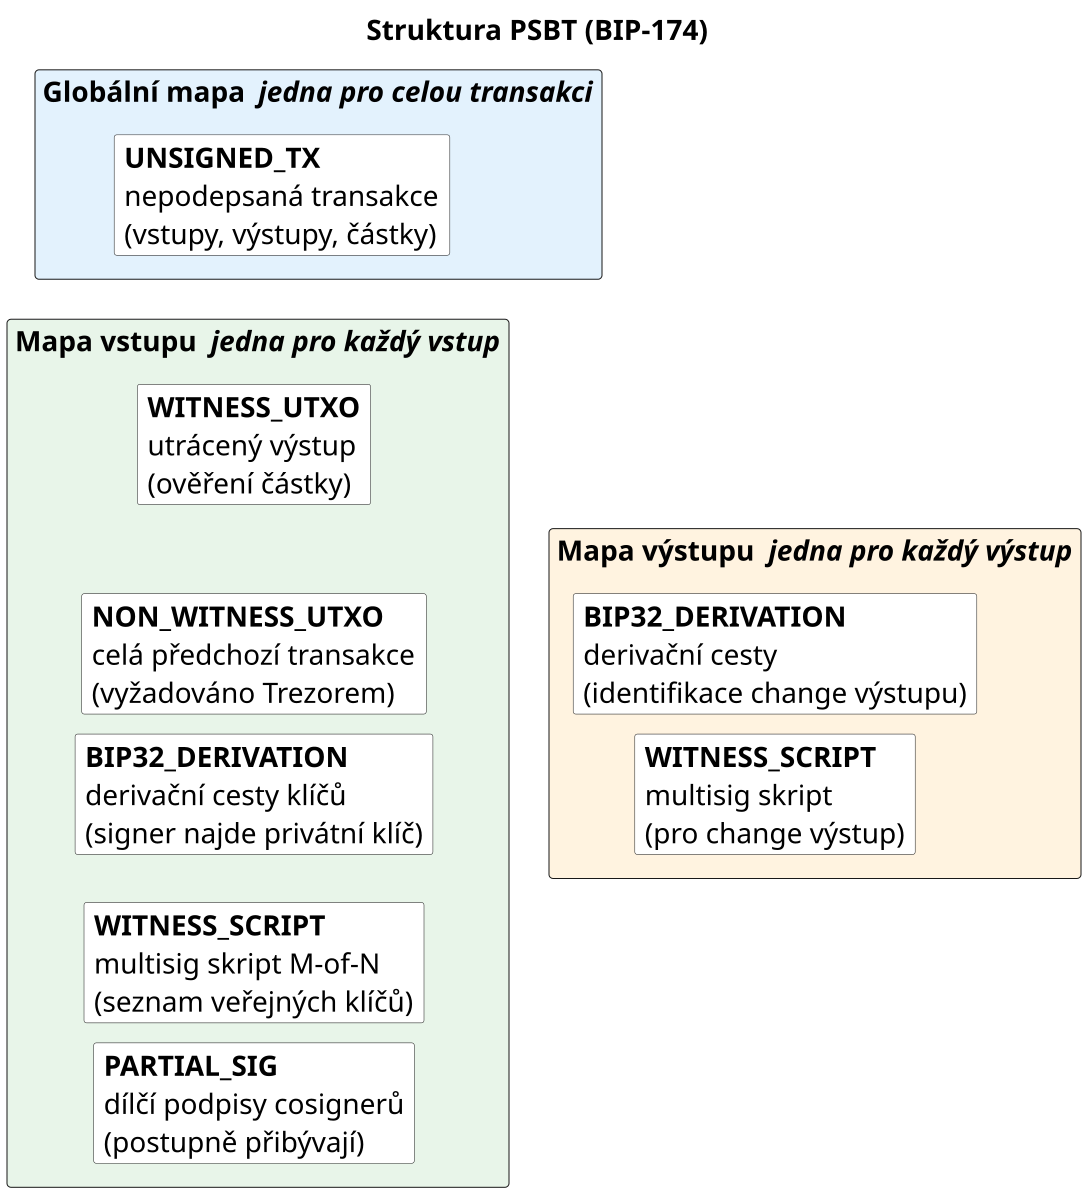
\includegraphics[width=\textwidth]{img/psbt-structure.pdf}
\caption{Struktura PSBT pro multisig transakci se dvěma vstupy a~dvěma výstupy.
Globální mapa obsahuje nepodepsanou transakci, mapy vstupů nesou data pro
podepisování a~mapa change výstupu obsahuje derivační cesty pro identifikaci
vlastního výstupu.}
\label{fig:psbt-structure}
\end{figure}

Standard rozlišuje šest rolí v~životním cyklu PSBT. Tyto role představují
logické kroky zpracování -- jedna entita může zastávat více rolí současně:
\begin{enumerate}
  \item \textbf{Creator} vytvoří PSBT s~globální transakcí (vstupy a~výstupy)
    a~prázdnými mapami vstupů a~výstupů.
  \item \textbf{Updater} doplní mapy o~metadata potřebná k~podpisu -- UTXO
    informace, derivační cesty, witness skripty. Po tomto kroku PSBT obsahuje
    vše, co signer potřebuje k~vytvoření podpisů.
  \item \textbf{Signer} na základě derivačních cest v~mapách vstupů najde
    příslušné privátní klíče a~přidá podpisy. V~rámci multisig schématu může
    PSBT projít postupně přes více signerů, z~nichž každý přidá svůj podpis.
  \item \textbf{Combiner} sloučí více částečně podepsaných PSBT (od různých
    signerů) do jednoho PSBT obsahujícího všechny podpisy.
  \item \textbf{Finalizer} zkontroluje, že všechny potřebné podpisy jsou
    přítomny, sestaví finální witness data a~odstraní pomocná metadata.
  \item \textbf{Extractor} extrahuje finální podepsanou transakci připravenou
    k~odeslání do sítě.
\end{enumerate}

Klíčovou vlastností PSBT je, že tyto role nemusí zastávat jedna entita --
naopak, celý smysl formátu spočívá v~rozdělení procesu podepisování mezi
více nezávislých systémů. Obrázek~\ref{fig:psbt-lifecycle} zachycuje
typický průběh zpracování PSBT pro multisig transakci.

\begin{figure}[htbp]
\centering
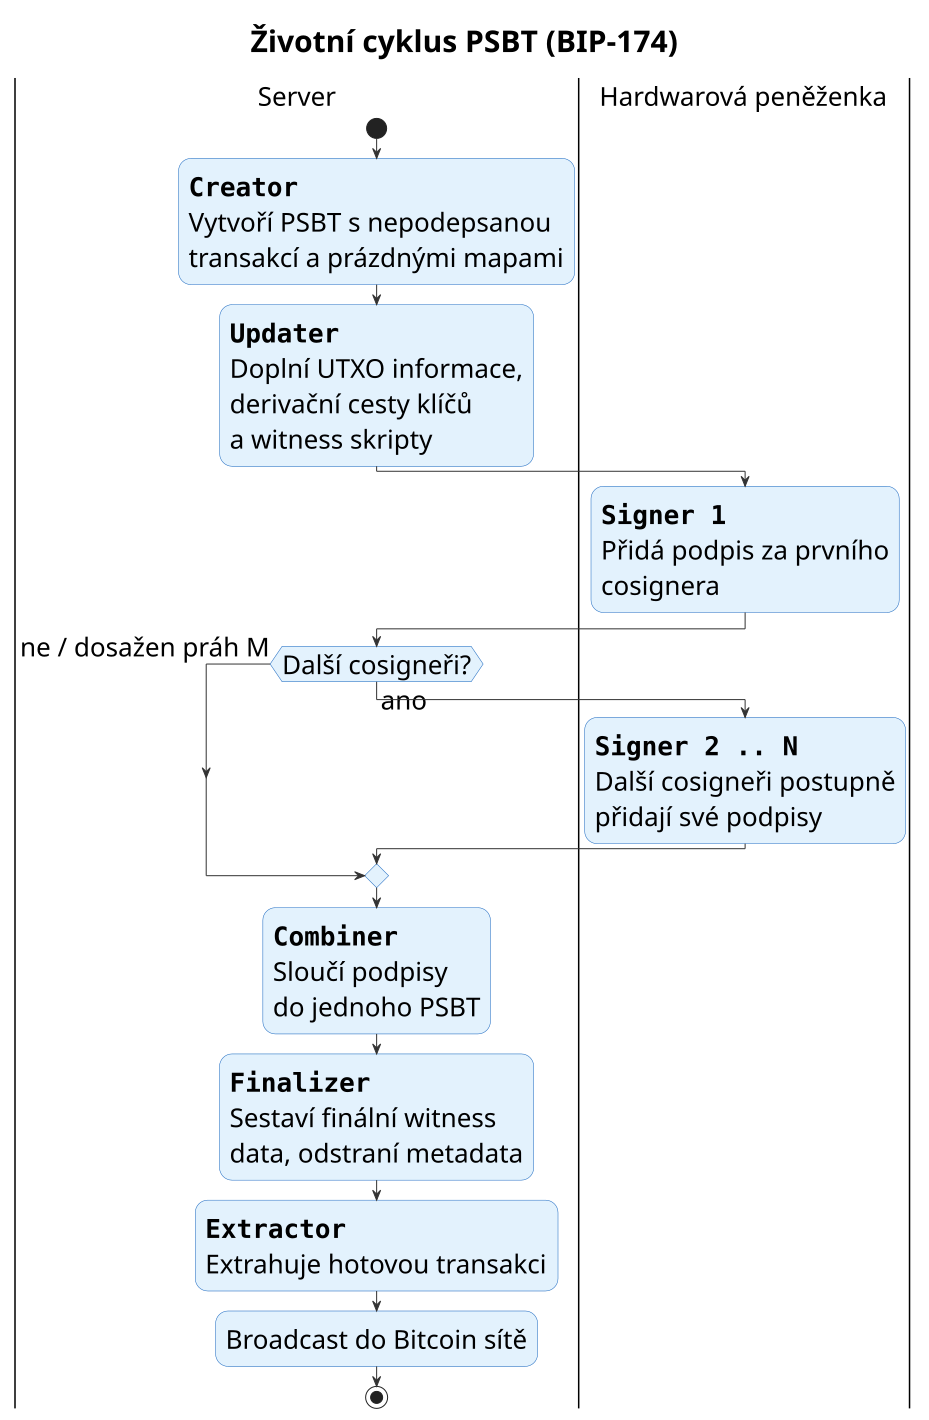
\includegraphics[width=0.85\textwidth]{img/psbt-lifecycle.pdf}
\caption{Životní cyklus PSBT pro multisig transakci. Serverová služba
zastává role Creator a~Updater, shromažďuje podpisy a~aktualizuje parametry
pro další cosignery. Trezor Connect interně provádí finalizaci (Combiner,
Finalizer) a~vrací kompletní serializovanou transakci (Extractor).
Hardwarové peněženky cosignerů vystupují jako Signeři.}
\label{fig:psbt-lifecycle}
\end{figure}

Celý proces probíhá následovně. Serverová služba nejprve vytvoří PSBT
s~nepodepsanou transakcí (\textbf{Creator}) -- na základě zvolených
UTXO vstupů, cílové adresy a~částky sestaví kostru transakce. Poté
do map vstupů doplní veškerá metadata potřebná k~podpisu
(\textbf{Updater}): referenční UTXO (aby signer mohl ověřit utrácené
částky), derivační cesty klíčů (aby hardwarová peněženka věděla, kterým
privátním klíčem podepsat), a~pro multisig vstupy i~kompletní witness
skript (aby signer znal seznam všech cosignerů a~požadovaný práh).
Do map výstupů přidá derivační cesty pro change výstup, aby peněženka
mohla ověřit, že vrácení změny směřuje zpět na vlastní adresu.

Takto připravené PSBT server odešle na mobilní aplikaci prvního
cosignera. Ta předá PSBT hardwarové peněžence (\textbf{Signer~1}),
která na svém displeji zobrazí detaily transakce -- cílovou adresu,
částku, poplatek. Po potvrzení uživatelem peněženka přidá svůj dílčí
podpis do polí \texttt{PARTIAL\_SIG} v~mapách vstupů. Částečně podepsané
PSBT se vrátí na server.

U~singlesig transakce je v~tomto okamžiku PSBT kompletní. U~multisig
transakce (např.\ 2-of-3) server čeká na podpis dalšího cosignera.
Druhý cosigner obdrží totéž PSBT (nyní již s~jedním podpisem), přidá
svůj podpis (\textbf{Signer~2}) a~PSBT se opět vrátí na server.

Jakmile server shromáždí požadovaný počet podpisů~$M$, předá je
poslednímu podepisujícímu Trezoru prostřednictvím Trezor Connect
parametrů. Trezor Connect interně provede sloučení podpisů
(\textbf{Combiner}), sestavení finální witness dat (\textbf{Finalizer})
a~extrakci kompletní podepsané transakce (\textbf{Extractor}),
kterou vrátí v~callback jako \texttt{serializedTx} připravenou
k~odeslání do Bitcoinové sítě.
Konkrétní mapování rolí na komponenty
systému popisujeme v~kapitole o~návrhu architektury.

\subsection{Výstupní deskriptory}
\label{sec:descriptors}

Výstupní deskriptory~\citep{BIP380} kompaktně popisují, jaké skripty
peněženka generuje. Pro multisig je podstatný formát z~BIP-383~\citep{BIP383}:

\begin{code}
wsh(sortedmulti(M,[fingerprint/path]xpub/0/*,...))
\end{code}

Tento deskriptor říká: \enquote{vytvořte P2WSH výstup obsahující M-of-N multisig
skript, kde jsou veřejné klíče seřazeny lexikograficky (dle BIP-67).} Každý
klíč je specifikován svým kořenovým otiskem (fingerprint), derivační cestou
a~rozšířeným veřejným klíčem (\texttt{xpub}). Suffix \texttt{/0/*} označuje
odvození přijímacích adres (resp.\ \texttt{/1/*} pro change adresy).

V~praxi to funguje tak, že uživatel vytvoří multisig peněženku
v~desktopové aplikaci (např.\ Sparrow Wallet~\citep{SparrowWallet}),
exportuje deskriptor a~vloží ho do mobilní peněženky. Z~deskriptoru
peněženka odvodí adresy, práh podpisů i~klíče cosignerů.


%%% -----------------------------------------------------------------
\section{Multisignature transakce}
\label{sec:multisig}

U~multisig transakcí je k~utracení prostředků potřeba M~podpisů z~N~klíčů
(schéma M-of-N). Oproti singlesig, kde zcizení jednoho klíče stačí ke ztrátě
prostředků, musí útočník u~multisig získat alespoň M~klíčů.

\subsection{Bezpečnostní výhody}
\label{sec:multisig-security}

Odpadá tak single point of failure. Praktické výhody:

\begin{itemize}
  \item \textbf{Ochrana proti krádeži}: Ani kompromitace jednoho klíče (např.\
    při zcizení hardwarové peněženky) neumožní útočníkovi provést transakci.
  \item \textbf{Odolnost proti ztrátě}: Ve schématu 2-of-3 může uživatel
    ztratit jeden klíč a~stále má dostatek klíčů k~obnovení přístupu
    k~prostředkům.
  \item \textbf{Geografická distribuce}: Jednotlivé klíče mohou být uloženy na
    různých místech, čímž se snižuje riziko současné ztráty.
\end{itemize}

\subsection{Případy užití}
\label{sec:multisig-usecases}

Multisig schémata nacházejí uplatnění v~různých scénářích:

\begin{itemize}
  \item \textbf{Sdílená správa} (shared custody): Schéma 2-of-3 umožňuje
    například rodinné správě prostředků, kde k~provedení transakce je potřeba
    souhlas alespoň dvou ze tří členů rodiny.
  \item \textbf{Dědění}: Pověřenec (právník, notář) drží jeden z~klíčů, který
    v~kombinaci s~klíčem dědice umožní přístup k~prostředkům po úmrtí majitele.
  \item \textbf{Firemní treasury}: Schéma 3-of-5 nebo vyšší zajišťuje, že
    firemní prostředky nemohou být odeslány bez souhlasu více odpovědných osob.
  \item \textbf{Osobní bezpečnost}: Jednotlivec uloží klíče 2-of-3 schématu do
    tří různých hardwarových peněženek na třech geograficky oddělených místech.
\end{itemize}

\subsection{Implementace pomocí P2WSH}
\label{sec:p2wsh-multisig}

V~současné implementaci Bitcoinu se nativní SegWit multisig transakce realizují
pomocí typu výstupu P2WSH~\citep{BIP141}. Výstupní skript obsahuje 32bajtový
SHA-256 hash tzv.\ witness skriptu, který definuje podmínky utrácení.

Pro M-of-N multisig má witness skript následující strukturu:
\begin{center}
\texttt{OP\_M <pubkey\_1> <pubkey\_2> ... <pubkey\_N> OP\_N OP\_CHECKMULTISIG}
\end{center}

Při utrácení takového výstupu musí witness data obsahovat M~validních podpisů
a~kompletní witness skript. Virtuální velikost vstupu multisig transakce je
výrazně větší než u~singlesig, což se projeví ve vyšších poplatcích.

Velikost vstupu ve virtuálních bajtech (vBytes) se dle
BIP-141~\citep{BIP141} vypočítá jako:
\[
  \text{vSize} = \text{base\_size} + \lceil \text{witness\_size} / 4 \rceil
\]
kde \emph{base\_size} je velikost newitness části vstupu (41~bajtů: outpoint
36~B, sequence 4~B a~délka skriptu 1~B) a~\emph{witness\_size} je velikost
witness dat. Pro M-of-N multisig vstup witness data obsahují: úvodní
\texttt{OP\_0} a~délky polí (přibližně 6~B), M~podpisů (každý maximálně
73~B: DER-kódovaný podpis 71--72~B plus push opcode) a~kompletní witness
skript s~N~veřejnými klíči (každý 34~B: 33~B komprimovaný klíč plus push
opcode). Celkově tedy:
\[
  \text{vSize}_{\text{input}} \approx 41 + \frac{6 + 73 \cdot M + 34 \cdot N}{4} \text{~vB}
\]
Například pro schéma 2-of-3 je odhadovaná velikost jednoho vstupu přibližně
$41 + (6 + 146 + 102)/4 \approx 105$~vB.


%%% -----------------------------------------------------------------
\section{Hardwarové peněženky}
\label{sec:hw-wallets}

Hardwarové peněženky uchovávají privátní klíče na izolovaném zařízení --
klíče ho nikdy neopouštějí. Na rozdíl od softwarových peněženek, kde jsou
klíče v~paměti počítače nebo telefonu a~hrozí jejich zcizení malwarem,
hardwarová peněženka podepisuje transakce ve vlastním prostředí. Uživatel
na displeji zařízení vidí adresu a~částku a~podepisování potvrdí fyzicky.

Na trhu existuje několik hardwarových peněženek s~podporou Bitcoinu.
Tyto peněženky se liší nejen hardwarem a~bezpečnostním modelem, ale
především \textbf{nemají jednotné rozhraní} pro komunikaci s~aplikacemi
třetích stran -- integrace s~každou peněženkou tak představuje
samostatnou implementační práci. Níže popisujeme nejrozšířenější
z~nich a~zdůvodňujeme volbu Trezoru.

\subsection{Trezor}
\label{sec:trezor}

Trezor, vyvinutý českou společností SatoshiLabs, patří mezi nejrozšířenější
hardwarové peněženky na trhu. Aktuální modelová řada zahrnuje několik zařízení
-- od Trezor Safe 3 přes Safe 5 s~barevným dotykovým displejem až po nejnovější
Safe 7, který jako první v~řadě podporuje bezdrátovou komunikaci
prostřednictvím Bluetooth a~NFC. Starší modely se připojují výhradně přes USB.
Všechna zařízení podporují protokol Bitcoin včetně SegWit a~multisig
transakcí.

Důležité je rozlišovat kompatibilitu s~mobilními zařízeními. Aplikace Trezor
Suite Mobile, která je nezbytná pro deeplink komunikaci, podporuje pouze novější
modely: Trezor Model~T, Safe~3, Safe~5 a~Safe~7. Starší model
\textbf{Trezor One} (první generace s~micro-USB konektorem) mobilní aplikaci
nepodporuje a~lze jej použít pouze s~desktopovou verzí Trezor Suite.
Pro testování a~provoz naší aplikace je tedy vyžadován minimálně Trezor Model~T.

Pro integraci s~aplikacemi třetích stran slouží rozhraní
\textbf{Trezor Connect}~\citep{TrezorConnect}. Toto API poskytuje
JavaScriptové rozhraní zprostředkovávající komunikaci mezi webovou nebo
mobilní aplikací a~hardwarovým zařízením. Na mobilních zařízeních Android
komunikace probíhá prostřednictvím \emph{deeplinků} -- speciálních URL,
které otevřou aplikaci Trezor Suite Mobile s~parametry transakce; po
potvrzení uživatelem na zařízení se podepsaná data vrátí zpět volající
aplikaci. Klíčové operace zahrnují \texttt{getPublicKey} (export
rozšířeného veřejného klíče pro danou derivační cestu) a~\texttt{signTransaction}
(podepsání transakce s~parametry specifickými pro daný typ výstupu).

\subsection{Ledger}
\label{sec:ledger}

Ledger je francouzský výrobce hardwarových peněženek s~modely Ledger Nano S
Plus, Nano X (s~Bluetooth) a~Ledger Stax. Zařízení používají proprietární
operační systém BOLOS běžící na bezpečnostním čipu (Secure Element).
Ledger podporuje Bitcoin včetně SegWit a~multisig.

Pro integraci s~aplikacemi třetích stran Ledger poskytuje Ledger Live SDK,
které však primárně cílí na webové a~desktopové aplikace. Na mobilních
zařízeních je komunikace možná přes Bluetooth (Nano X), avšak vyžaduje
implementaci vlastního transportního protokolu. Ledger neposkytuje
deeplink API srovnatelné s~Trezor Connect, což komplikuje integraci
z~mobilních aplikací třetích stran.

\subsection{Coldcard}
\label{sec:coldcard}

Coldcard od kanadské společnosti Coinkite je hardwarová peněženka zaměřená
výhradně na Bitcoin. Je navržena pro maximální bezpečnost -- podporuje
plně \emph{air-gapped} provoz, kdy zařízení nikdy nemusí být připojeno
k~počítači ani telefonu. Transakce se přenášejí prostřednictvím microSD
karty ve formátu PSBT.

Coldcard neposkytuje žádné API ani SDK pro přímou komunikaci z~mobilní
aplikace. Integrace je možná pouze přes manuální přenos PSBT souborů
(microSD nebo NFC u~novějších modelů), což je pro mobilní peněženku
s~automatizovaným workflow nevhodné.

\subsection{BitBox02}
\label{sec:bitbox02}

BitBox02 od švýcarské společnosti Shift Crypto je kompaktní hardwarová
peněženka s~dotykovými senzory pro potvrzování transakcí. Zařízení
komunikuje přes USB-C a~nabízí open-source firmware.

Pro integraci BitBox02 poskytuje vlastní SDK komunikující přes WebSocket
protokol a~USB HID. Mobilní SDK existuje, ale je primárně určeno pro
vlastní aplikaci BitBoxApp. Integrace z~aplikace třetí strany na Androidu
by vyžadovala implementaci USB HID komunikace a~proprietárního protokolu.

\subsection{Shrnutí a volba Trezoru}

Z~uvedených hardwarových peněženek Trezor jako jediný poskytuje deeplink
API umožňující mobilní aplikaci třetí strany iniciovat podepisování
bez implementace nízkoúrovňového komunikačního protokolu. Ledger vyžaduje
vlastní Bluetooth transport, Coldcard je navržen pro offline přenos
a~BitBox02 vyžaduje USB HID komunikaci. Trezor je navíc v~České republice
zdaleka nejrozšířenější hardwarovou peněženkou, což odpovídá cílovému
publiku této práce.


%%% -----------------------------------------------------------------
\section{Přehled existujících řešení}
\label{sec:existing-solutions}

Níže srovnáváme sedm existujících peněženek z~hlediska podpory multisig
transakcí, coin control a~integrace s~hardwarovými peněženkami.

\subsection{Trezor Suite}
\label{sec:trezor-suite}

Trezor Suite~\citep{TrezorSuite} je oficiální aplikace od společnosti
SatoshiLabs pro správu prostředků na zařízeních Trezor. Je dostupná jako
desktopová aplikace pro Windows, macOS a~Linux, jako webová aplikace
a~v~mobilní verzi Trezor Suite Mobile pro Android a~iOS.

Aplikace nabízí přehledné uživatelské rozhraní, správu více účtů, plnou
podporu coin control s~vizualizací UTXO a~integraci s~burzami pro nákup
a~prodej kryptoměn. Trezor Suite podporuje všechny typy SegWit adres včetně
P2WPKH a~Taproot.

\textbf{Omezení}: Trezor Suite neposkytuje nativní správu multisig peněženek.
Uživatel nemůže v~aplikaci vytvořit multisig konfiguraci, importovat
deskriptor ani koordinovat podepisování s~více cosignery. Pro multisig
transakce je nutné použít aplikaci třetí strany (např.\ Electrum nebo Sparrow),
která komunikuje se zařízením Trezor prostřednictvím Trezor Connect. Mobilní
verze Trezor Suite Lite navíc nabízí pouze omezenou podmnožinu funkcí
desktopové verze.

\subsection{Sparrow Wallet}
\label{sec:sparrow}

Sparrow Wallet~\citep{SparrowWallet} je desktopová Bitcoin peněženka zaměřená
na bezpečnost, transparentnost a~pokročilé funkce. Aplikace je dostupná pro
Windows, macOS a~Linux a~je vydávána pod open-source licencí Apache 2.0.

Sparrow nabízí pravděpodobně nejkomplexnější podporu multisig transakcí ze
všech analyzovaných řešení. Uživatel může přímo v~aplikaci vytvořit multisig
konfiguraci M-of-N s~libovolnou kombinací klíčů -- z~hardwarových peněženek
různých výrobců (Trezor, Ledger, Coldcard, aj.), ze softwarových klíčů nebo
z~importovaných \texttt{xpub} klíčů. Aplikace generuje výstupní deskriptor,
který lze exportovat pro použití v~jiných peněženkách.

Další silné stránky zahrnují detailní coin control s~možností manuálního
označování (labeling) UTXO, vizualizaci transakčního grafu, analýzu soukromí,
podporu PSBT a~možnost připojení k~vlastnímu Bitcoin uzlu nebo serveru Electrum.

\textbf{Omezení}: Sparrow Wallet je dostupný \emph{výhradně jako desktopová
aplikace}. Neexistuje mobilní verze pro Android ani iOS. Uživatel, který chce
spravovat svou multisig peněženku mimo dosah stolního počítače, nemá tuto
možnost.

\subsection{Liana}
\label{sec:liana}

Liana~\citep{LianaWallet} je peněženka vyvíjená společností Wizardsardine,
která využívá jazyk Miniscript pro definici pokročilých podmínek utrácení.
Hlavní inovací je podpora \emph{časově zamčené obnovy} (timelocked recovery) --
uživatel může definovat záložní klíč, který se aktivuje po uplynutí zadaného
časového intervalu, pokud primární klíč nebyl použit.

Tento přístup řeší problém dědění a~obnovy bez nutnosti důvěry třetí straně.
Liana podporuje integraci s~hardwarovými peněženkami Ledger a~některými dalšími
zařízeními.

\textbf{Omezení}: Liana je dostupná pouze jako desktopová aplikace. Mobilní
verze neexistuje. Podpora hardwarových peněženek nezahrnuje zařízení Trezor,
což ji činí nepoužitelnou pro uživatele, kteří svou infrastrukturu klíčů
postavili na zařízeních Trezor. Multisig v~tradičním smyslu (M-of-N) není
primárním zaměřením aplikace -- místo toho se Liana soustředí na Miniscript
politiky, které mohou být pro běžného uživatele obtížně srozumitelné.

\subsection{BlueWallet}
\label{sec:bluewallet}

BlueWallet~\citep{BlueWallet} je open-source mobilní peněženka dostupná pro
Android a~iOS. Nabízí přehledné uživatelské rozhraní a~širokou škálu funkcí
včetně podpory Lightning Network.

BlueWallet obsahuje funkci \emph{Multisig Vault}, která umožňuje vytvoření
multisig peněženky přímo v~mobilní aplikaci. Uživatel může definovat schéma
M-of-N a~přidat klíče ze seed frází nebo importovaných \texttt{xpub} klíčů.
Aplikace rovněž podporuje coin control s~možností zmrazení (freeze) jednotlivých
UTXO a~export/import PSBT.

\textbf{Omezení}: Integrace s~hardwarovými peněženkami je omezená na komunikaci
prostřednictvím QR kódů nebo sdílení souborů PSBT. BlueWallet nepodporuje
přímé propojení s~Trezorem přes USB nebo deeplink protokol. Proces podepisování
s~hardwarovou peněženkou je tak vícekrokový a~vyžaduje manuální přenos dat
mezi aplikacemi, což zhoršuje uživatelský komfort a~zvyšuje riziko chyb.

\subsection{Nunchuk}
\label{sec:nunchuk}

Nunchuk~\citep{Nunchuk} je peněženka navržená primárně pro multisig správu
Bitcoinu. Je dostupná jako mobilní aplikace pro Android a~iOS i~jako desktopová
aplikace. Nunchuk podporuje širokou škálu hardwarových peněženek včetně Trezor,
Ledger, Coldcard a~BitBox.

Aplikace nabízí intuitivní průvodce vytvořením multisig peněženky, správu
klíčů s~možností testování podpisů (health check), kolaborativní podepisování
přes cloud synchronizaci a~podporu coin control. Nunchuk rovněž implementuje
koncept \emph{inheritance planning} s~využitím časových zámků.

\textbf{Omezení}: Pokročilé funkce Nunchuku, včetně kolaborativního
podepisování, air-gapped klíčů a~inheritance planningu, jsou dostupné pouze
v~rámci placeného předplatného (Nunchuk Premium). Bezplatná verze omezuje počet
klíčů a~peněženek. Tento model předplatného může být překážkou pro uživatele,
kteří preferují plně otevřená řešení bez závislosti na službách třetí strany.
Navíc cloudová synchronizace, byť end-to-end šifrovaná, přidává závislost
na~externí infrastruktuře provozovatele.

\subsection{Electrum}
\label{sec:electrum}

Electrum~\citep{Electrum} je jedna z~nejstarších a~nejpoužívanějších
Bitcoinových peněženek, aktivně vyvíjená od roku 2011. Desktopová verze nabízí
kompletní sadu pokročilých funkcí: multisig peněženky s~libovolným schématem
M-of-N, detailní coin control, integraci s~hardwarovými peněženkami (Trezor,
Ledger, Coldcard), podporu PSBT, Lightning Network a~připojení k~vlastnímu
Electrum serveru.

\textbf{Omezení}: Electrum má sice verzi pro Android, ta však nabízí výrazně
omezenou funkčnost oproti desktopové verzi. Mobilní verze nepodporuje multisig
peněženky, integraci s~hardwarovými peněženkami ani coin control. Uživatel je
tak na mobilním zařízení omezen na základní singlesig operace, což výrazně
snižuje hodnotu mobilní verze pro naše cílové použití.

\subsection{Wasabi Wallet}
\label{sec:wasabi}

Wasabi Wallet~\citep{WasabiWallet} je desktopová Bitcoin peněženka zaměřená
především na ochranu soukromí uživatele. Její hlavní funkcí je implementace
protokolu CoinJoin (ve variantě WabiSabi), který umožňuje společné míchání
transakcí více uživatelů za účelem ztížení analýzy blockchainu.

Wasabi nabízí automatický výběr UTXO optimalizovaný pro soukromí, integraci
s~Tor sítí pro anonymní komunikaci a~přehledné označování prostředků podle
úrovně soukromí (red/yellow/green shielding).

\textbf{Omezení}: Wasabi Wallet je dostupná \emph{výhradně jako desktopová
aplikace} pro Windows, macOS a~Linux. Mobilní verze neexistuje. Aplikace rovněž
nepodporuje multisignature transakce -- zaměřuje se výhradně na singlesig
operace s~důrazem na soukromí. Pro uživatele hledající kombinaci multisig
a~mobilní platformy tak Wasabi nepředstavuje řešení.


%%% -----------------------------------------------------------------
\section{Srovnání a identifikace nedostatků}
\label{sec:comparison}

Tabulka~\ref{tab:wallet-comparison} shrnuje klíčové vlastnosti analyzovaných
peněženek.

\begin{table}[htbp]
\centering
\caption{Srovnání existujících Bitcoinových peněženek}
\label{tab:wallet-comparison}
\footnotesize
\begin{tabular}{|l|c|c|c|c|c|c|}
\hline
\textbf{Peněženka} & \textbf{Desk.} & \textbf{Mobil} & \textbf{Multisig} & \textbf{Coin ctrl} & \textbf{HW peněž.} & \textbf{Licence} \\
\hline
Trezor Suite   & Ano & Ano\textsuperscript{*} & Ne  & Ano & Trezor    & Propriet. \\
Sparrow        & Ano & Ne                      & Ano & Ano & Více      & Apache~2.0 \\
Liana          & Ano & Ne                      & Část.\textsuperscript{$\dagger$} & Ne  & Jiné & MIT \\
BlueWallet     & Ne  & Ano                     & Ano & Ano & QR/PSBT   & MIT \\
Nunchuk        & Ano & Ano                     & Ano & Ano & Více      & Propriet.\textsuperscript{$\ddagger$} \\
Electrum       & Ano & Ano\textsuperscript{*}  & Ano\textsuperscript{*} & Ano\textsuperscript{*} & Více & MIT \\
Wasabi         & Ano & Ne                      & Ne  & Ano & Ne        & MIT \\
\hline
\textbf{Naše řeš.} & Ne & \textbf{Ano} & \textbf{Ano} & \textbf{Ano} & \textbf{Trezor} & --- \\
\hline
\end{tabular}
\normalsize

\smallskip
\footnotesize
\textsuperscript{*}~Mobilní verze s~omezenou funkcionalitou. \\
\textsuperscript{$\dagger$}~Miniscript politiky namísto tradičního M-of-N multisig. \\
\textsuperscript{$\ddagger$}~Pokročilé funkce vyžadují placené předplatné. \\
\normalsize
\end{table}

Ze srovnání vyplývá:

\begin{enumerate}
  \item \textbf{Desktopová řešení dominují v~pokročilých funkcích}:
    Nejkomplexnější multisig podporu nabízejí Sparrow a~Electrum, obě primárně
    desktopové aplikace. Sparrow, který považujeme za referenční řešení
    z~hlediska UX multisig workflow, nemá vůbec mobilní verzi.

  \item \textbf{Mobilní řešení mají omezenou integraci s~HW peněženkami}:
    BlueWallet sice podporuje multisig na mobilu, ale komunikace s~hardwarovou
    peněženkou probíhá pouze přes QR kódy a~manuální sdílení PSBT souborů,
    bez přímé integrace přes deeplink nebo USB.

  \item \textbf{Nunchuk se nejvíce blíží cílové specifikaci}, avšak jeho
    obchodní model s~placeným předplatným pro pokročilé funkce a~závislost na
    cloudové synchronizaci představují omezení pro uživatele, kteří preferují
    plně otevřené a~nezávislé řešení.

  \item \textbf{Žádné existující řešení nekombinuje} na platformě Android
    nativní multisig správu, coin control a~přímou integraci s~hardwarovou
    peněženkou Trezor prostřednictvím Trezor Connect API.
\end{enumerate}

Tato mezera je hlavní motivací pro aplikaci navrhovanou v~této práci,
která nabídne:

\begin{itemize}
  \item Plnou podporu multisignature transakcí ve schématu M-of-N s~využitím
    standardu BIP-174~\cite{BIP174} (PSBT) pro koordinaci podepisování.
  \item Integraci s~hardwarovou peněženkou Trezor prostřednictvím Trezor
    Connect API a~deeplink protokolu, bez nutnosti manuálního přenosu dat.
  \item Funkci coin control umožňující uživateli ručně vybírat UTXO při tvorbě
    transakcí.
  \item Bezpečnostní model, ve kterém privátní klíče nikdy neopouštějí
    hardwarové zařízení a~serverová část systému pracuje výhradně
    s~veřejnými klíči.
\end{itemize}

%%% -----------------------------------------------------------------
\section{Analýza technických přístupů}
\label{sec:analyza-pristupu}

Předchozí sekce identifikovaly mezeru na trhu -- absenci mobilní Bitcoinové
peněženky, která by kombinovala multisig správu, coin control a~přímou
integraci s~hardwarovou peněženkou Trezor. Než přistoupíme ke specifikaci
požadavků, je nutné analyzovat technické přístupy ke klíčovým problémům,
které implementace takové aplikace přináší. Tato sekce rozebírá tři
hlavní rozhodnutí: jakým způsobem komunikovat s~hardwarovým zařízením,
jak řešit správu multisig peněženek a~jaký formát zvolit pro koordinaci
podepisování. U~každého rozhodnutí uvádíme zvažované alternativy, jejich
výhody a~nevýhody a~zdůvodňujeme zvolenou variantu.


\subsection{Komunikace s~hardwarovou peněženkou Trezor}
\label{sec:analyza-trezor}

Zásadní architektonickou otázkou je, jakým způsobem bude mobilní aplikace
na platformě Android komunikovat se zařízením Trezor za účelem podepisování
transakcí. Identifikovali jsme tři přístupy.

\subsubsection{Trezor Connect JavaScript SDK}

Oficiální integrační rozhraní Trezor Connect~\citep{TrezorConnect} je
distribuováno jako JavaScriptová knihovna (\texttt{@trezor/connect}), určená
pro prostředí webového prohlížeče a~Node.js. Knihovna abstrahuje veškerou
komunikaci se zařízením do jednoduchých volání -- vývojář zavolá funkci
\texttt{signTransaction} s~parametry transakce a~SDK se postará o~sestavení
USB zpráv, obsluhu stavového automatu i~zobrazení potvrzovacího dialogu.

Pro nativní platformu Android však oficiální SDK neexistuje. V~repozitáři
SatoshiLabs se nachází archivovaná Android knihovna, která ale neodpovídá
aktuálnímu firmware zařízení, nepokrývá novější typy transakcí (včetně
P2WSH multisig) a~není aktivně udržovaná. Tento přístup je proto pro
nativní Android aplikaci nepoužitelný.

\subsubsection{Přímá USB komunikace přes Android USB Host API}

Technicky je možné komunikovat se zařízením Trezor přímo prostřednictvím
Android USB Host API -- tedy stejným způsobem, jakým to interně dělá
aplikace Trezor Suite Mobile. Zařízení Trezor se na úrovni USB chová
jako HID zařízení a~komunikuje pomocí zpráv ve formátu Protocol Buffers.

Podepisování Bitcoinové transakce na Trezoru však není jednorázová
operace. Zařízení má omezenou paměť (řádově jednotky kilobajtů pro
pracovní data), a~proto nemůže přijmout celou transakci najednou.
Místo toho probíhá vícekrokový dialog mezi aplikací a~zařízením:

\begin{enumerate}
  \item Aplikace odešle zprávu \texttt{SignTx} s~počtem vstupů a~výstupů.
  \item Zařízení odpoví zprávou \texttt{TxRequest}, ve které si vyžádá
    konkrétní data -- například vstup č.~2 nebo kompletní předchozí transakci
    odkazovanou vstupem č.~0.
  \item Aplikace odpovídá zprávou \texttt{TxAck} s~požadovanými daty.
  \item Kroky 2--3 se opakují v~desítkách iterací, dokud zařízení nezíská
    všechna potřebná data a~nevygeneruje podpisy.
\end{enumerate}

\noindent
Implementace tohoto přístupu by vyžadovala:

\begin{itemize}
  \item \textbf{USB transportní vrstvu} -- protokol pracuje s~64bajtovými
    pakety, zprávy je nutné fragmentovat a~sestavovat.
  \item \textbf{Protocol Buffers definice} -- kompletní sada zpráv
    odpovídající aktuálnímu firmware (desítky typů zpráv).
  \item \textbf{Stavový automat podepisování} -- implementaci výše
    popsaného cyklu \texttt{SignTx}~$\to$~\texttt{TxRequest}~$\to$~\texttt{TxAck}
    včetně zpracování všech typů požadavků (vstupy, výstupy, předchozí
    transakce, metadata).
  \item \textbf{Multisig rozšíření} -- pro multisig transakce je navíc
    nutné předávat witness skripty a~derivační cesty všech cosignerů
    s~korektním řazením klíčů dle BIP-67~\citep{BIP67}.
\end{itemize}

\noindent
Hrubý odhad pracnosti je přibližně 20 pracovních dní. Zdrojový kód
aplikace Trezor Suite je sice veřejně dostupný, ale je publikován pod
licencí T-RSL (Trezor Restricted Source License)~\citep{TRSL}, která
explicitně zakazuje kopírování kódu do jiných projektů -- umožňuje
pouze čtení za účelem studia. Implementace by proto musela vzniknout
zcela od základu na základě veřejné dokumentace
protokolu~\citep{TrezorFirmwareDocs}.

\subsubsection{Deeplink protokol přes Trezor Suite Mobile}

Třetí možností je delegovat komunikaci se zařízením na aplikaci Trezor
Suite Mobile, která je na cílovém Android zařízení nainstalována. Mobilní
aplikace otevře Trezor Suite Mobile prostřednictvím deeplinku (speciální
URL schéma), předá parametry transakce (vstupy, výstupy, referenční
transakce) a~registruje adresu pro zpětné volání. Po potvrzení uživatelem
na displeji hardwarové peněženky Trezor Suite Mobile vrátí podepsaná data
zpět volající aplikaci prostřednictvím callback URL.

Výhodou tohoto přístupu je využití produkčně otestovaného a~průběžně
udržovaného kódu od SatoshiLabs, který pokrývá veškerou složitost USB
protokolu, stavového automatu i~podporu všech typů transakcí. Nevýhodou
je závislost na instalaci externí aplikace a~krátké přesměrování
uživatele mimo peněženku.

\subsubsection{Zhodnocení a volba}

Přímá USB komunikace by přinesla lepší uživatelský zážitek -- celý
proces podepisování by probíhal uvnitř jedné aplikace bez přepínání
kontextu. Představuje však přibližně 20~dní dodatečného vývoje
a~nutnost implementace složitého protokolu zcela od základu (kvůli
licenčním omezením). JavaScript SDK je pro Android nepoužitelné.
V~kontextu rozsahu bakalářské práce je delegování na Trezor Suite
Mobile prostřednictvím deeplinků pragmatickou volbou.

Architektura aplikace je navržena s~čistým interním rozhraním pro
podepisování (\emph{signing interface}), za kterým se v~aktuální verzi
skrývá deeplink komunikace s~Trezor Suite Mobile. Toto rozhraní
umožňuje v~budoucnu přidat přímou USB komunikaci jako alternativní
implementaci bez nutnosti změn ve zbytku systému.


\subsection{Správa multisig peněženek}
\label{sec:analyza-multisig}

Druhým klíčovým rozhodnutím je, jakým způsobem bude multisig peněženka
vytvořena a~nakonfigurována. Vytvoření multisig peněženky je netriviální
koordinační úloha -- je nutné:

\begin{enumerate}
  \item Shromáždit rozšířené veřejné klíče (\texttt{xpub}) od všech
    N~cosignerů, přičemž každý cosigner musí klíč exportovat ze svého
    vlastního hardwarového zařízení.
  \item Dohodnout se na parametrech peněženky: práhu M~(kolik podpisů
    je potřeba k~utracení), derivačních cestách dle BIP-48~\citep{BIP48}
    a~typu skriptu (P2WSH).
  \item Z~těchto parametrů vygenerovat výstupní deskriptor a~ověřit,
    že všichni cosigneři pracují se shodnou konfigurací.
  \item Odvodit sadu multisig adres a~ověřit je na blockchainu.
\end{enumerate}

Na desktopové platformě tento proces pokrývá Sparrow
Wallet~\citep{SparrowWallet} -- nabízí průvodce vytvořením multisig
peněženky, umožňuje přidávat klíče z~hardwarových peněženek různých
výrobců (Trezor, Ledger, Coldcard), generuje a~validuje deskriptory
a~exportuje je pro použití v~jiných peněženkách.

Implementace celého konfiguračního procesu přímo v~mobilní aplikaci
by vyžadovala: bezpečný protokol pro výměnu \texttt{xpub} klíčů mezi
cosignery (potenciálně přes QR kódy, NFC nebo síťovou komunikaci),
uživatelské rozhraní pro přidávání, odebírání a~verifikaci cosignerů,
a~generování deskriptorů s~validací dle BIP-380~\citep{BIP380}
a~BIP-383~\citep{BIP383}. Jedná se o~funkcionalitu, která by svým
rozsahem odpovídala samostatnému projektu.

Zvolený přístup proto odděluje \emph{konfiguraci} peněženky od
jejího \emph{provozu}. Uživatel vytvoří multisig peněženku
v~desktopové aplikaci (typicky Sparrow Wallet, který je open-source
pod licencí Apache~2.0), exportuje výstupní deskriptor ve
standardizovaném formátu \texttt{wsh(sortedmulti(...))} a~vloží
ho do mobilní aplikace. Z~deskriptoru aplikace odvodí všechny
potřebné parametry -- práh, klíče cosignerů, derivační cesty --
a~může začít s~provozem: zobrazováním zůstatků, vytvářením
transakcí, koordinací podepisování a~broadcastem.

Tento kompromis je záměrný. Konfigurace multisig peněženky se
provádí typicky jednou a~vyžaduje přístup ke všem cosignerům
současně. Provozní operace (odesílání, podepisování, sledování
stavu) se provádějí opakovaně a~právě pro ně je mobilní aplikace
nejpřínosnější.


\subsection{Koordinace podepisování pomocí PSBT}
\label{sec:analyza-psbt}

V~multisig schématu musí tutéž transakci postupně podepsat více cosignerů,
potenciálně na různých zařízeních a~v~různém čase. Klíčovou otázkou je,
v~jakém formátu transakci mezi cosignery distribuovat a~jak sbírat
dílčí podpisy.

\subsubsection{Vlastní formát}

Jednou z~možností je definovat vlastní datový formát (například JSON),
který by obsahoval parametry transakce a~pole pro podpisy. Tento přístup
by umožnil maximální flexibilitu, ale přinesl by zásadní nevýhodu:
ztrátu interoperability. Žádná jiná peněženka by nedokázala takový formát
zpracovat, a~uživatel by byl zcela závislý na jedné aplikaci pro celý
životní cyklus transakce.

\subsubsection{Standard PSBT (BIP-174)}

Standard PSBT (Partially Signed Bitcoin Transaction,
BIP-174~\citep{BIP174}), jehož strukturu jsme popsali
v~sekci~\ref{sec:psbt}, je navržen přesně pro tento účel. PSBT
je podporován hardwarovými peněženkami Trezor (prostřednictvím Trezor
Connect~\citep{TrezorConnect}), desktopovými peněženkami
Sparrow~\citep{SparrowWallet} a~Electrum~\citep{Electrum} i~dalšími
nástroji Bitcoinového ekosystému.

Volba PSBT zajišťuje, že aplikace zapadá do existujícího ekosystému.
Uživatel může například zahájit transakci v~mobilní aplikaci, exportovat
částečně podepsanou PSBT a~dokončit podepisování ve Sparrow na desktopu
-- nebo naopak. Tato interoperabilita je pro multisig workflow obzvláště
důležitá, neboť jednotliví cosigneři mohou používat různé peněženky.

Z~těchto důvodů volíme PSBT jako formát pro koordinaci podepisování.
Backendová služba vystupuje jako koordinátor: vytvoří PSBT s~kompletními
metadaty (role Creator a~Updater), distribuuje ji cosignerům k~podpisu,
sbírá dílčí podpisy a~po dosažení prahu~M provede finalizaci
a~broadcast do sítě.


\subsection{Shrnutí: rozsah vlastní implementace}
\label{sec:analyza-rozsah}

Na základě předchozí analýzy lze shrnout rozdělení odpovědností.
Aplikace \emph{sama implementuje}: konstrukci a~finalizaci PSBT
(BIP-174), derivaci adres z~veřejných klíčů (BIP-32), správu UTXO
a~coin control, odhad transakčních poplatků, koordinaci multisig
podepisování a~celé uživatelské rozhraní pro Android.
Aplikace \emph{deleguje}: vytváření multisig peněženek na desktopovou
aplikaci (Sparrow Wallet), podepisování transakcí na hardwarovou
peněženku Trezor prostřednictvím Trezor Suite Mobile a~přístup
k~blockchainovým datům na veřejná API (Blockstream Esplora
pro mainnet, Mempool.space pro testnet4).

Toto rozdělení odráží rozsah realizovatelný v~rámci bakalářské práce
a~přitom poskytuje kompletní a~použitelnou aplikaci pokrývající celý
operační cyklus -- od příjmu prostředků přes tvorbu a~koordinaci
transakcí až po broadcast do Bitcoinové sítě. Architektura je navržena
tak, aby delegované části (zejména podepisování) mohly být v~budoucnu
nahrazeny vlastní implementací bez zásahu do zbytku systému.

Na základě provedené analýzy nyní v~následující kapitole specifikujeme
požadavky na systém.
